\documentclass[12pt]{iopart}
\usepackage{graphicx}
\usepackage{epstopdf}
\graphicspath{{figure/}}
\usepackage{color}
\usepackage{bm}
\usepackage{ulem}
\usepackage[colorlinks,linkcolor=blue,anchorcolor=blue,citecolor=blue,urlcolor=blue]{hyperref}
\usepackage{indentfirst}

\begin{document}
\title[]{Laser-driven collisionless shock acceleration in confined plasmas}

\author{H. He$^1$, }
\address{$^1$ Center for Applied Physics and Technology, HEDPS, State Key Laboratory of Nuclear Physics and Technology, and School of Physics, Peking University, Beijing, 100871, China}
\ead{bqiao@pku.edu.cn}

\date{\today}

\begin{abstract}


\end{abstract}

\pacs{}

\maketitle
\section{INTRODUCTION}
\label{Introduction}
Since 2000, a great resea rch effort has been devoted to producing laser-driven ion beams\cite{daido_review_2012,macchi_ion_2013} which are oriented to vast promising applications including tumor therapy, proton imaging, nuclear fusion, neutron source generation, and high energy density science. And several ion acceleration mechanisms are proposed, such as target normal sheath acceleration (TNSA), radiation pressure acceleration (RPA), hole-boring acceleration (HBA), collisionless shock acceleration (CSA), magnetic vortex acceleration (MVA), etc. 

By the most studied TNSA mechanism, the foil is irradiated by intense laser whose energy is delivered to the electrons with J×B heating. Then ions are accelerated in the sheath field created by those superthermal electrons at the rear of the foil. Some applications, such as proton imaging and neutron source generation, are achieved by this concept. While TNSA is proved experimentally robust, its ion beams are charactered with large divergence and exponential energy spectrum, which limiting its efficiency and uses in other applications. Also studied a lot is the RPA mechanism which employs circular polarized laser to directly push the electrons with light pressure. And the whole plasma foil is accelerated as a “light-sail”. RPA is theoretically much more efficient and can produce beams with narrow energy spread. However, rigorous requirement in both laser and target condition make it difficult to practically apply RPA.

Benefited by nowadays high intensity large energy lasers, as well as great advancement in manufacture of near-critical plasma, alternative ion acceleration concepts may have chance to be realized in experiments. Among them, CSA is a promising mechanism which produces high-flux quasi-monoenergetic ion beams. Theoretic and numeric studies show that CSA has several advantages over TNSA or RPA, for specific, ion energy scaling linearly with laser intensity, relax requirement on laser condition, and high repetition rate. For experimental study, quasi-monoenergetic 1 MeV ion beam has been achieved by CSA with CO2 laser facility which, however, limited by its low intensity. In CSA, the ponderomotive force of laser pushes near-critical plasma to pile up a high-density spike. When the density ratio of spike and unperturbed plasma exceeds specific threshold (2.56)\cite{zhang_quasi-monoenergetic_2016}, a collisionless electrostatic shock is exited and propagates with a constant velocity vs. As the plasma density jumps abruptly, a strong charge separation field is established at the shock front where upstream ions are reflected and accelerated to 2vs.

In previous researches on CSA, shocks are mostly considered in one- or quasi-one-dimensional configuration. Namely, either periodic boundary or very large laser focal spot is used. However, this one-dimensional approximation is unfair in experiments, because small focal spot is required for high laser intensity. On the opposite, shock must propagate a long-distance for efficient ion acceleration. When shock propagation distance is much larger than laser focal size, transverse effects must be considered. As shown in this paper, finite laser focal size has important impact on the CSA scheme, which may stand in the way of implementation of CSA experiments. 

We find that multi-dimension effect the 1D scheme in three aspects. Firstly, the high density downstream region local within laser spot size is prone to extent to non-irradiated region, which lowers its density when shock propagates and finally extinguishes the shock. Secondly, the superthermal electrons, essential for heating upstream plasma, diverts to ambient region, which lead to lower temperature and consequently lower shock velocity. Thirdly, intense laser usually filaments when propagates in near-critical plasma. These filaments easily get through the peak of density spike and greatly perturb the upstream, which distort the shock front and spoil the quality of ion beams. To mitigate these effects, it’s necessary to couple the near-critical plasma to proper confinements. Here, we propose and demonstrate by PIC simulations that a metal tube[See Fig.\ref{fig:sketch}] as the confinement can far improve both shock and ion beam quality.

\begin{figure}
    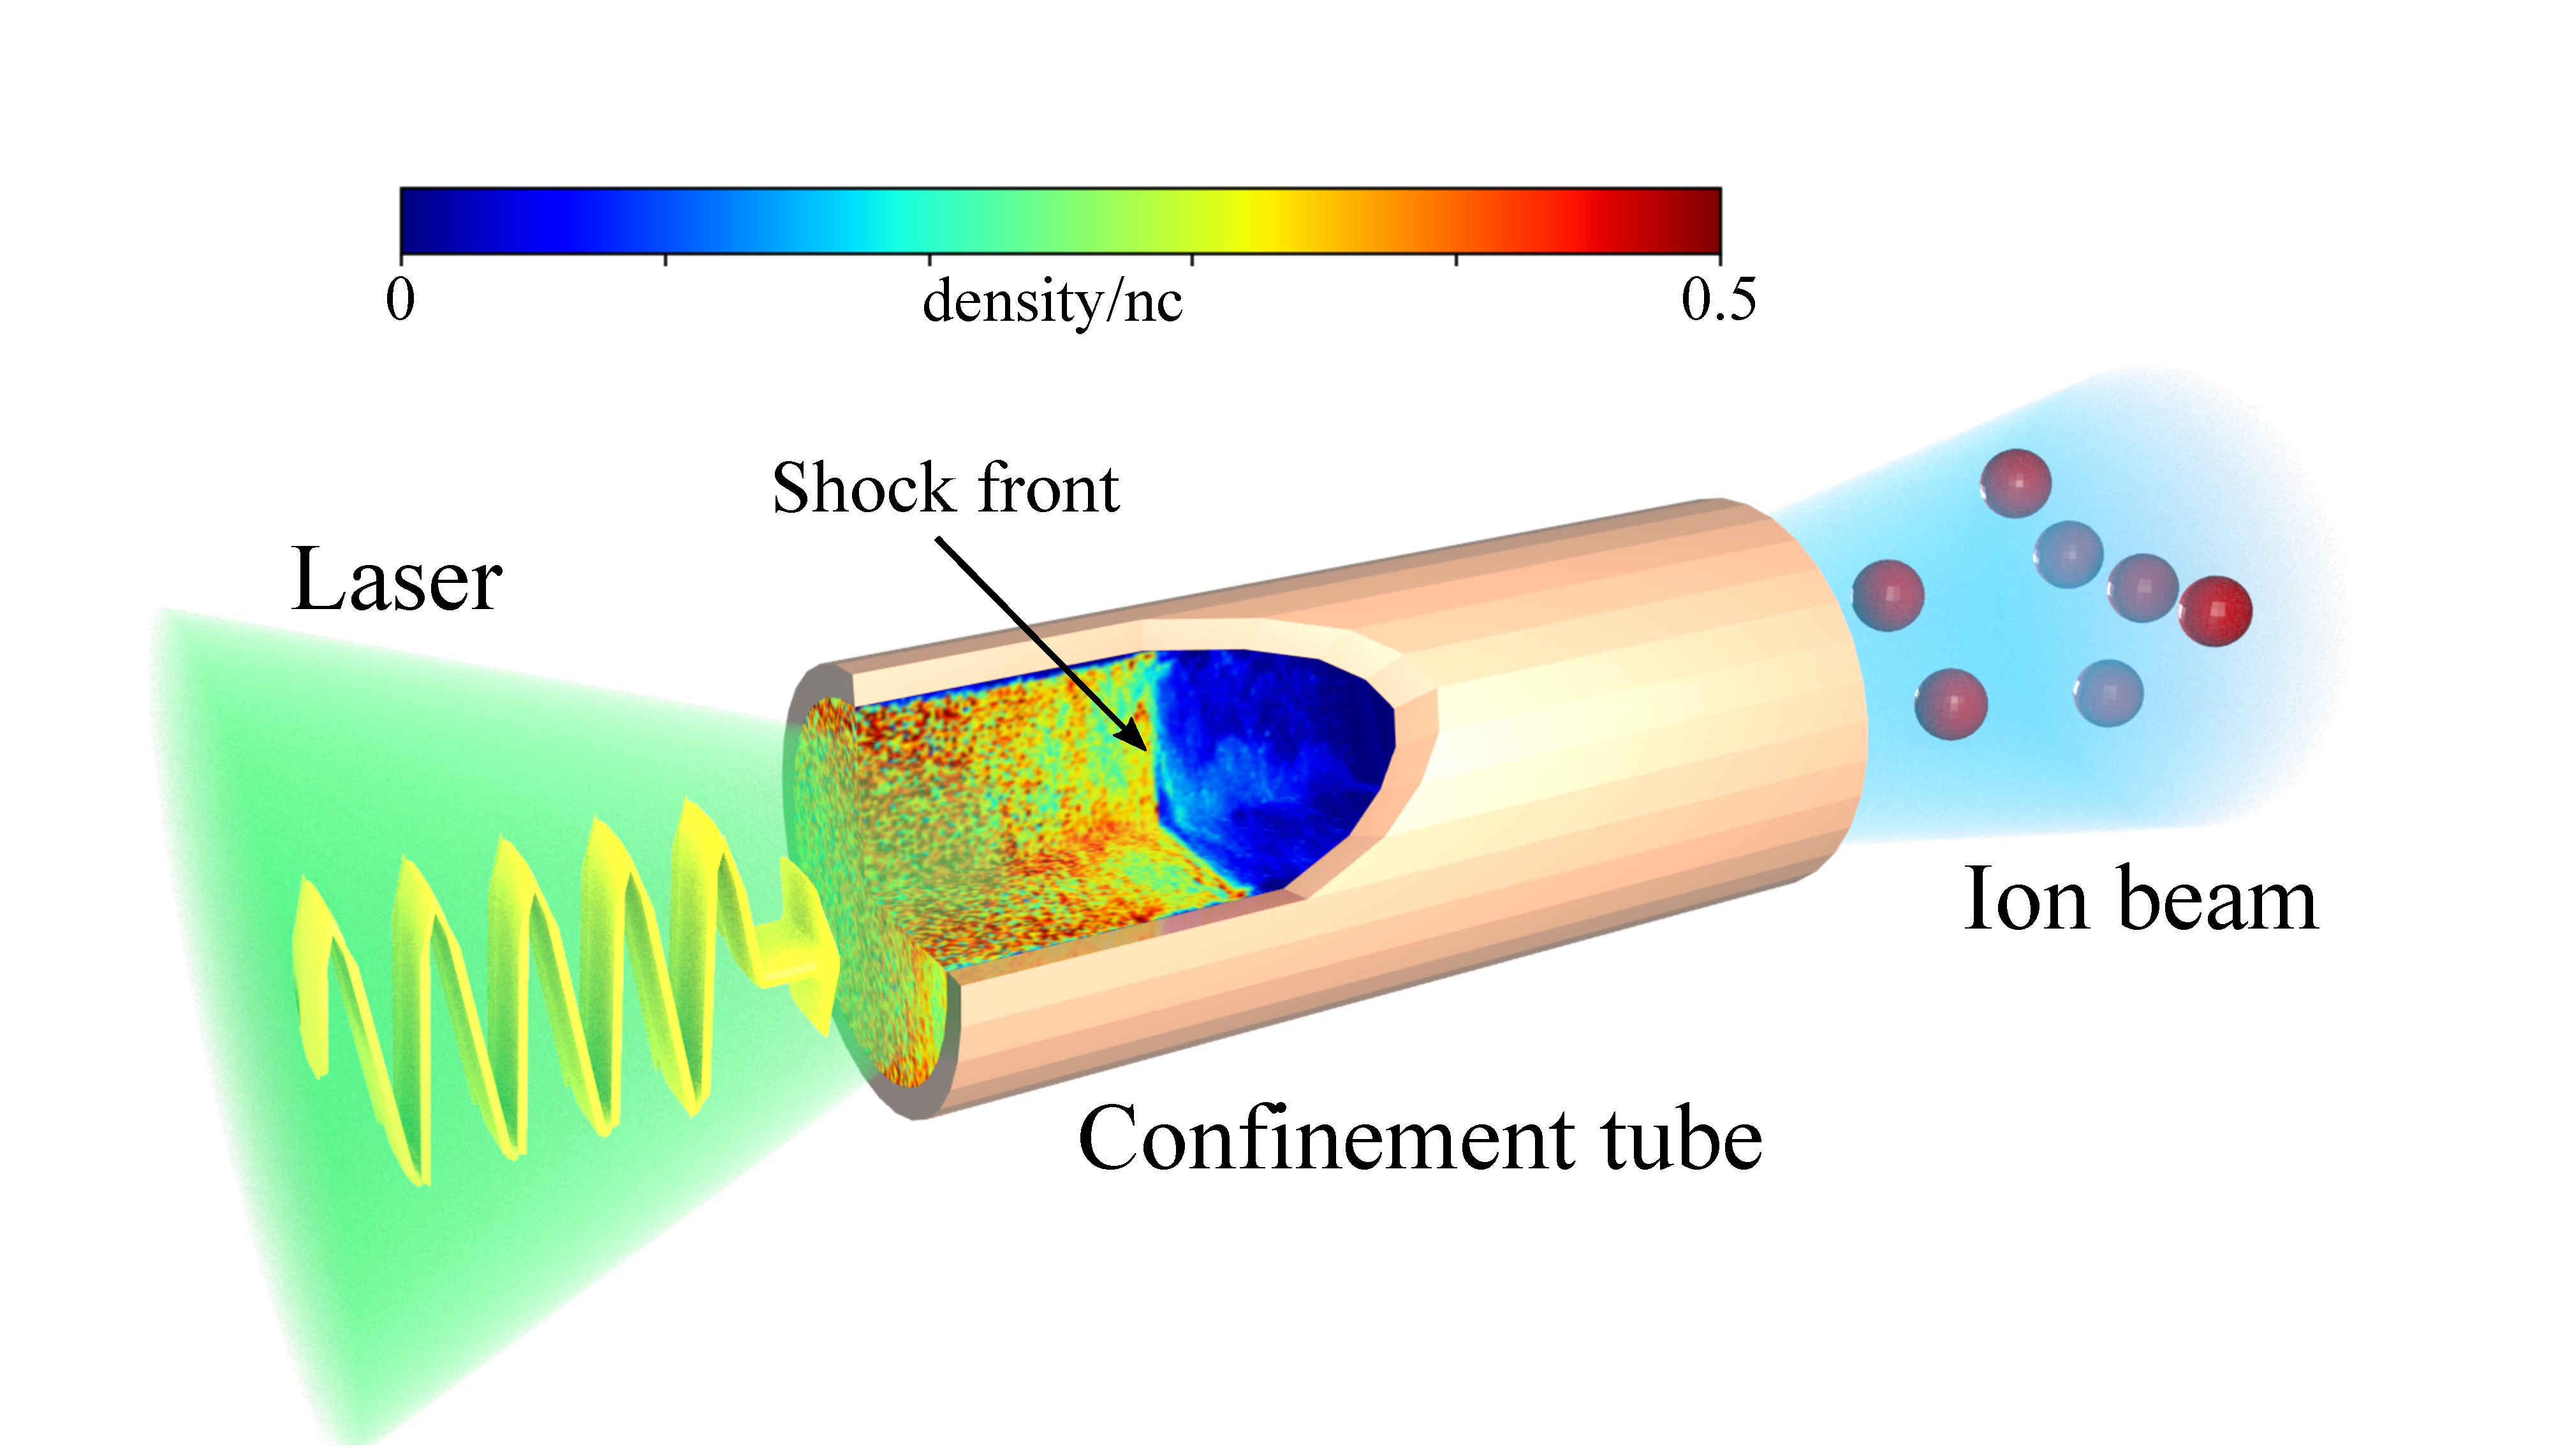
\includegraphics[width=8cm]{sketch.eps}\label{fig:sketch}
    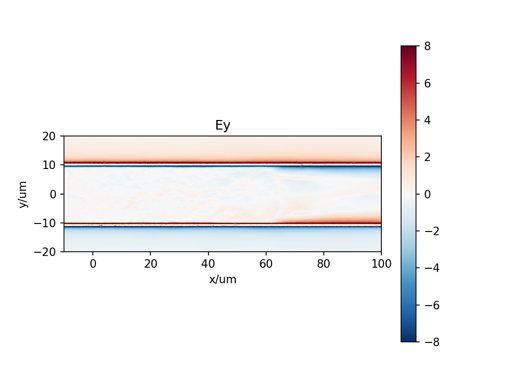
\includegraphics[width=8cm]{confine_ey.png} \label{fig:confine_ey}
    \caption{(color online) (a) Schematic of the proposed confinement scheme, where near-critical plasma is confined in a high density high-Z tube. (b) Electrons in tube are heated by divergent superthermal electrons, and forming a confinement bipolar electric fied Ey around the tube wall.}
\end{figure}

In this paper, firstly, we point out some effects that could undermine the acceleration process by two-dimensional PIC simulation. Following that, we propose a confined-configuration to mitigate those effects. And the advance of the confined- over open-configuration is discussed. Finally, a new easy method of controlling plasma density profile is displayed by simulation. 
 
\section{Transverse effects on CSA}
\label{theory}
 
In the one-dimensional model, laser irradiated at the near-critical plasma is reflected at critical density surface. As a result, the ponderomotive force of laser pushes the critical surface forward at velocity $\frac{v_{hb}}{c}=\sqrt{\frac{Z m}{M}\frac{n_c}{n_e}\frac{(2-\eta)\cos\theta}{4}\frac{I_{18} \lambda_{\mu}^2}{1.37}}$ termed hole-boring velocity\cite{gibbon_short_2005}. As critical surface moves, it swaps plasma along the way and piles up a high-density spike. This process creates the essential condition for launching a collisionless shock, namely, a density jump between spike and unperturbed plasma. The threshold of shock formation is obtained by kinetic analysis\cite{fiuza_laser-driven_2012}, where density ratio to be 2.56\cite{zhang_quasi-monoenergetic_2016}. After shock launches, it propagates at constant velocity $v_{s}$, or equally Mach number $M=v_s/c_s$, where $c_s=\sqrt{T_e/M}$ is the ion-acoustic velocity in upstream\cite{tidman_shock_1971}. The density jump at the shock front also generate strong electrostatic field which forms a potential barrier. In the frame of shock, upstream ions moving relatively to the shock front are reflected by this potential barrier. Backing to laboratory frame, those ions are accelerated to $2v_s$. Each gains energy of $\epsilon=2m_i v_s^2$.  This ion acceleration progress continues until shock become slower than critical velocity due to energy loss. Therefore, so long as shock keeps propagating stably, CSA could efficiently produce quasi-monoenergetic ion beams.

As shock is expected to propagate far beyond the focal size, transverse effects become signifiant. When shock moves forward, downstream plasma extents transversely and lowers its density. Additionally, superthermal electrons heated by laser's $\vec{J}\times \vec{B} $ absorption\cite{gibbon_short_2005} diverts and results in lower upstream temperature. We next estimate the significance of those effects and their impact on CSA. To begin with, it is assumed that 1D model still applies shortly after shock forming. So by 1D electrostastic hydro-dynamic model\cite{tidman_shock_1971,zhang_quasi-monoenergetic_2016} we have $M=\sqrt{N_2 / N_1}<1.6$, where the subscript ``1(2)'' denote quantities in upstream(downstream) plasma. 

\begin{figure}[htbp]
    \centering
    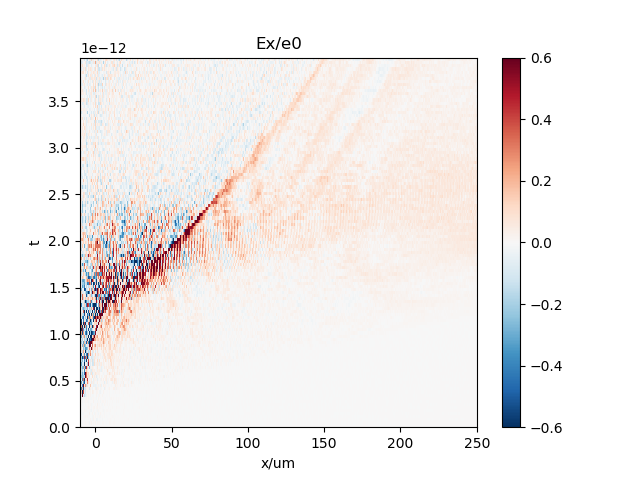
\includegraphics[width=7cm]{ex_trace.png}\label{fig:open_ex_track}
    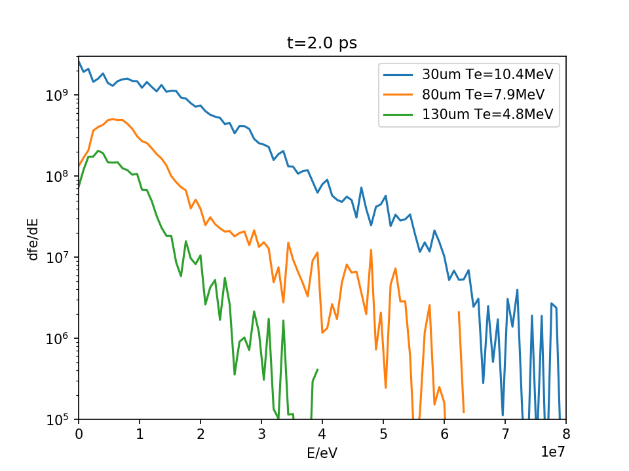
\includegraphics[width=7cm]{Te_x.png}\label{fig:open_Te}
    \caption{(color online)(a) Time evolution of the longitudinal electric field. The red line indicates the track of shock front with large $E_x$. Shock launches at about $30\mu m$, and extinguishes beyond $80/mu m$. (b) Local electron energy spectrum. Temperature is measured with the slope of the local distribution in interval as width as the spot and of $30/mu m$ in length. Temperature is droping along with longitudinal distance.}
\end{figure}

For the effect of lowering downstream density, $N_2$ can be roughly estimated in 2D by $\tilde{N_2}=N_2 \cdot d_f\big/(d_f+L)$, where $d_f$ is the focal spot size, and $L$ is the length of transverse extention. If downstream plasma uniformly extents at ion acoustic velocity, $L=c_s\Delta t$. It's also reasonable to infer that shock extinguishes when the density jump is canceled which means $\tilde{N_2}=N_1$. So by simple algebra, the time of shock extinguishing reads $\Delta t=d_f/c_s(N_2/N1-1)$. Then we obtain the limit distance within which shock can propagate, $s_{lim}=v_s \cdot \Delta t=d_fM(M^2-1)$. It is indenpendent on electron temperature $T_e$, because the higher $T_e$ the slower shock propagates, but also the slower downstream plasma extents. Using $d_f=20\mu m,M=1.6$, we easily get $s_{lim}\approx 50\mu m$. This result is fair consist with our simulation [Fig.\ref{fig:open_ex_track}].

Concerning the effect of divergence of superthermal electrons, we assuming divergence angle to be $\theta=45^\circ$  \cite{gibbon_short_2005}. And it is obvious that upstream temperature is proportional to the energy density carried by superthermal electrons. So in 2D case, electron temperature can be expressed as $T_e\propto E_e/d_f$, where $E_e$ is the total energy converted from laser to hot electrons. At distance $s$, it is the same $\tilde{T_e} \propto E_e/(d_f+s\tan{\theta})$. And we obtain the temperature ratio $\tilde{T_e}/T_e=d_f/(d_f+s\cdot\tan{\theta})$. Using above result $s=s_{lim}$, we find more than $70\%$ temperature lost in upstream plasma[Fig.\ref{fig:open_Te}], which causes the same portion of energy lost in accelerated ions.

\section{CSA in confined configuration}
\label{confined}

We compare in detail the confined and un-confined cases to demonstrate the differences between them by 2D PIC simulations using EPOCH code\cite{arber_contemporary_2015}. 
In un-confined cases simulation box is set to be $500\mu m \times 60\mu m$ with $11$grids$/\mu m$ in each direction. And 16 electrons/ions are used per grid. Open boundary condition is used in transverse direction. P-polarized laser with $\lambda=1\mu m$ and intensity $I_0=8.78\times 10^{19}W/cm^2$(or normalized amplitude $a_0 = 8$) is incidented from left edge. The planar laser has a gaussian temporal profile with duration $\tau=1ps$. Laser spot is supergaussian $I(r)=I_0\exp(-(r/r_0)^8)$ giving a FWHM radius of $20\mu m$.

In quasi-1D case, simulation box is set to be $500\mu m \times 60\mu m$ with $11$grids$/\mu m$ in each direction. And 16 electrons/ions are used per grid. Periodic boundary condition is used in transverse direction. P-polarized laser with $\lambda=1\mu m$ and intensity $I_0=8.78\times 10^{19}W/cm^2$(or normalized amplitude $a_0 = 8$) is incidented from left edge. The laser has a gaussian temporal profile with duration $\tau=1ps$. In 2D case, most sets are the same other than borden box of $500\mu m \times 100\mu m$ and open boundary condition in transverse direction. The box is bordened to avoid unnecessary boundary effects on the main physical area. Laser focal spot is set supergaussian $I(r)=I_0\exp(-(r/r_0)^8)$ giving a FWHM radius of $10\mu m$.

Plasma is composed of hydrogen ions($H^+$) and electrons. The optimal tailored density profile for CSA along shock propagation is studied in previous researches\cite{fiuza_ion_2013,fiuza_laser-driven_2012,boella_numerical_2017}. We use the similar one consist of a rapid $10\mu m$ linear rising and a slow exponential declining with $20\mu m$ scale length. The rapid rising is necessary to maximize ponderomotive force of laser to pile up density spike. And the slow declining is necessary for keeping the quality of ion energy spectrum which, otherwise, would be ruined by TNSA sheath field. The declining can also compensate the density jump  of shock when shock losses energy to ions and slows down.\cite{macchi_solitary_2012}. 


\section{Discussion}
\label{discussion}


\section{Conclusion}
\label{conclusion}
 
\ack


\section*{References}
\bibliography{refers}
\bibliographystyle{iopart-num}

\end{document}